\documentclass[12pt]{article}
\usepackage{fullpage,amsmath,amsfonts,mathpazo,microtype,nicefrac,graphicx,fancyhdr,listings,hyperref,csvsimple}

\usepackage[english]{babel}
\usepackage[utf8]{inputenc}

\author{Akhil Ketkar Arjun Sanghvi \\
	\texttt{akhilketkar@g.harvard.edu} \texttt{asanghvi@g.harvard.edu}}

% \pagestyle{fancy}
% \rhead{AM205 2014 Final Project -- AK AS}


% include graphics
% \includegraphics[width=0.8\textwidth]{figureProb40}

% include code 
% 

% include csv
% \csvautotabular{charge_output.csv}


\title{Spectral Analysis of Enron Email Data}
\begin{document}
\maketitle
\section{Introduction} \indent The Enron email dataset is interesting because it contains real email data from employees at a major organization that was involved in a massive fraud. The dataset contains a large amount of information that can be used to answer a number of interesting questions in areas such as Social Network Analysis and Organizational Behavior, such as: who are the key actors in the information network, are there communities in within the network, how do features of a network evolve over time, does information flow over a network look different in a "crisis" etc. 

\section{Brief Background on Enron}
	The Enron timeline taken from an article published by the New York Times \cite{nyt} \\
	
	1985 - Houston Natural Gas merges with InterNorth to form Enron, HNG CEO Kenneth Lay becomes CEO of combined company the following year.

1989 - Enron begins trading natural gas commodities.

1990 - Lay hires Jeffrey Skilling to lead the company's effort to focus on commodities trading in the deregulated markets. Andrew S. Fastow is one of Skilling's first hires later that year.

1991 - Richard Causey leaves Arthur Andersen LLP to join Enron as assistant controller.

1997 - Skilling named president and chief operating officer of Enron. Fastow creates Chewco, a partnership, to buy the University of California pension fund's stake in another joint venture dubbed JEDI, but Chewco doesn't meet requirements to be kept off Enron's balance sheet. First step toward similar financial moves to hide debt and inflate profits that fuel Enron's downfall.

1998 - Fastow named finance chief.

1999- Causey named chief accounting officer. Fastow creates the first of two partnerships, LJM, purported to "buy" poorly performing Enron assets and hedge risky investments but really helps the company hide debt and inflate profits. Enron directors approve Fastow's plan that he run the partnerships that do deals with Enron while continuing as Enron's finance chief. Causey and former chief risk officer Rick Buy assigned to monitor such deals to protect Enron's interests.

August 2000 - Enron shares reach high of 90.

December 2000 - Enron announces that Skilling, then president and chief operating officer, will succeed Kenneth Lay as CEO in February 2001. Lay will remain as chairman. Stock hits 52-week high of 84.87. \\

2001:

Aug. 14 - Skilling resigns; Lay named CEO again.

Aug. 22 - Finance executive Sherron Watkins meets privately with Lay to discuss concerns of murky finance and accounting that could ruin the company.

Oct. 16 - Enron announces 638 million in third-quarter losses and a 1.2 billion reduction in shareholder equity stemming from writeoffs related to failed broadband and water trading ventures as well as unwinding of so-called Raptors, or fragile entities backed by falling Enron stock created to hedge inflated asset values and keep hundreds of millions of dollars in debt off the energy company's books.

Oct. 19 - Securities and Exchange Commission launches inquiry into Enron finances.

Oct. 22 - Enron acknowledges SEC inquiry into a possible conflict of interest related to the company's dealings with Fastow's partnerships. Lay says, "We will cooperate fully with the SEC and look forward to the opportunity to put any concern about these transactions to rest."

Oct. 23 - Lay professes confidence in Fastow to analysts.

Oct. 24 - Fastow ousted.

Nov. 5 - Enron treasurer Ben Glisan Jr. and in-house attorney Kristina Mordaunt fired for investing in Fastow-run partnership. Each invested 5,800 in 2001 and received a 1 million return a few weeks later.

Nov. 8 - Enron files documents with SEC revising its financial statements for previous five years to account for 586 million in losses.

Nov. 9 - Dynegy Inc. announces an agreement to buy Enron for more than 8 billion in stock.

Nov. 19 - Enron restates its third-quarter earnings and discloses a 690 million debt is due Nov. 27.

Nov. 28 - Enron stock plunges below 1 as Dynegy Inc. aborts its plan to buy its former rival.

Dec. 2 - Enron goes bankrupt, thousands of workers laid off.
	

\section{Data and Resulting Graphs}
	\subsection{Dataset}
	There are several versions of the Enron email dataset. The version that we are utilizing for this paper comes from the work of Jitesh Shetty and Jafar Adibi \cite{shetty} at ISI. Shetty and Adibi cleaned the dataset by dropping emails that were blank, duplicates of unique emails, had junk data, or were returned by the system due to transaction failures. The final dataset consists of 252,759 emails in 3000 user defined folders from 151 people. Shetty and Abidi loaded the information into a MySql database that contains four tables containing information about the employees, messages, recipients and reference information. We chose this version of the dataset mainly because it is has been structured into a relational database. Unfortunately Shetty and Adibi's website (which was used as a source by a number of papers) was taken down recently. So we retrieved a copy of the the data from Joel Pfeiffer's \cite{pfeiffer}. In addition to the email data, we also used data on the positions and specific roles of various employees from Youngser Park\cite{park}. \par
	We made several modifications to the dataset to arrive at the version that was used in the analysis. Some of the changes were normalizing the email addresses for all the employees, adding missing emails addresses, removing emails that were not sent from other employees etc. We then incorporated the employee position data into the email data to create the final version of the dataset. 
	\subsection{Graphs}
	All subsequent analysis in the paper relies on the network representation of the dataset mentioned above. The nodes of the network are the employees of Enron and the edges represent individual email exchanges. Certain parts of the paper use directed graphs where an edge goes from a sender to the receiver of the email while other parts use undirected graphs where an edge simply denotes an email sent between the two nodes.
	\par
	Here is an example of the network drawn from emails sent in October 2000. In this period Enron's share price was close to it's all time highs. \\
	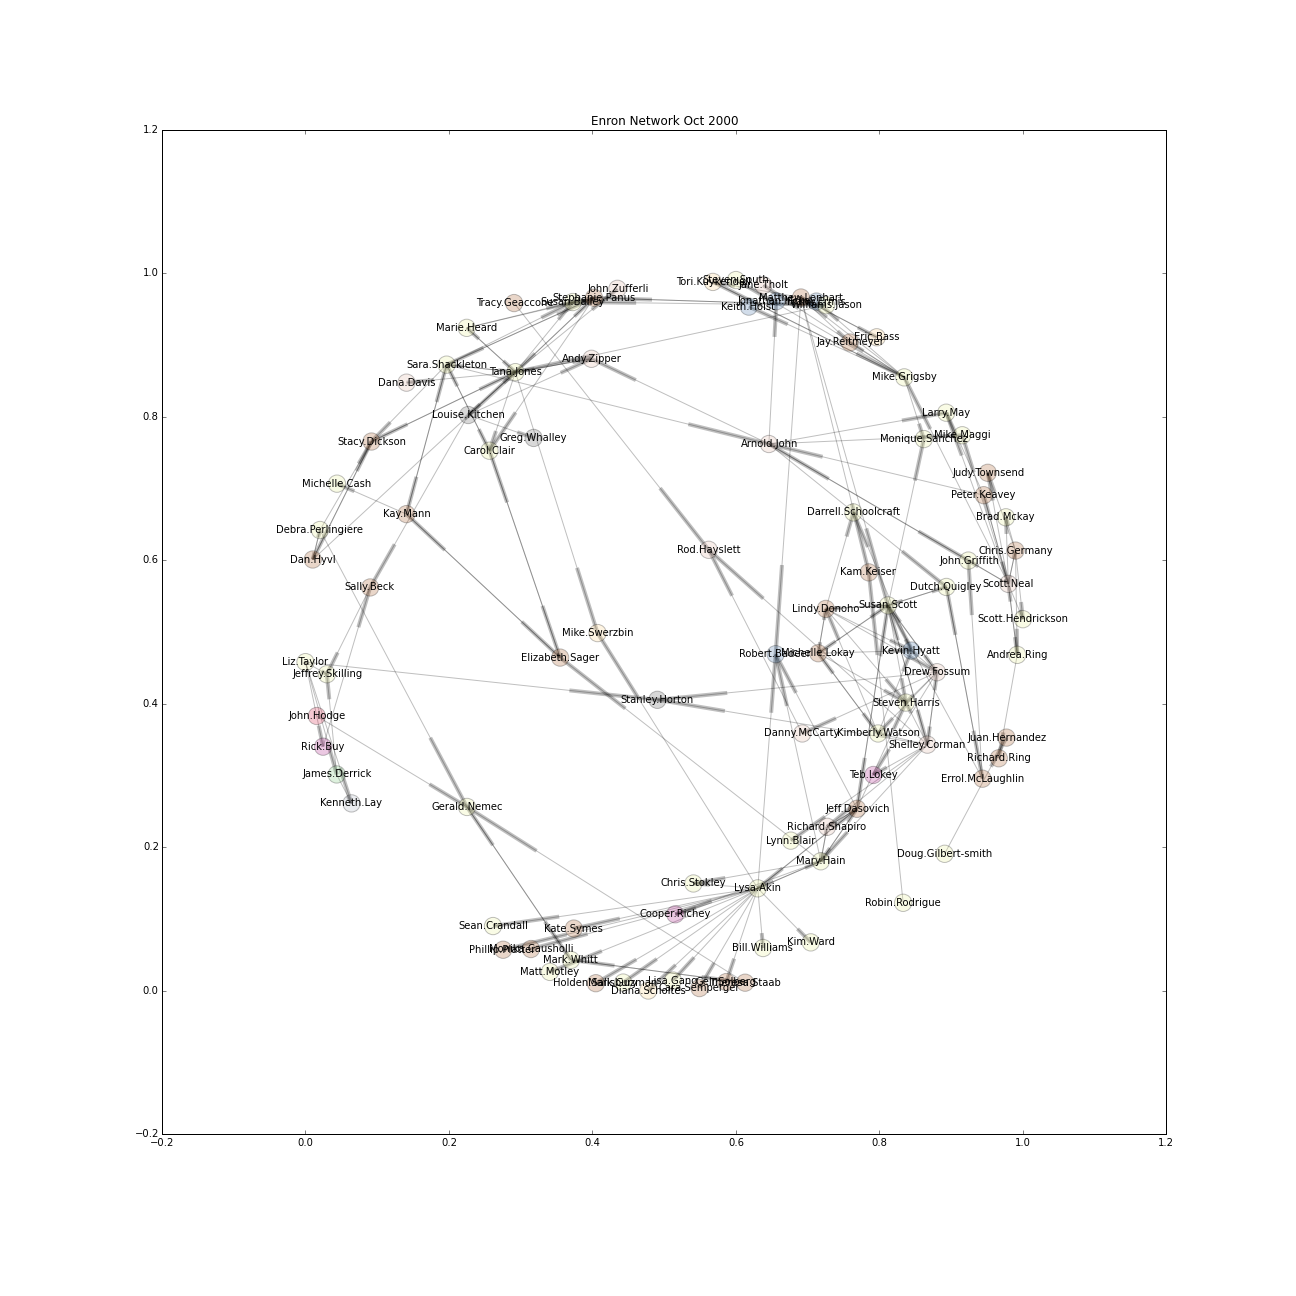
\includegraphics[width=1\textwidth]{figureEnronOct2000}
	\\
	Compare the network in Oct 2000 to this network created from emails sent in October 2001 at which point the fraud at Enron has been exposed and Enron is nearing bankruptcy.
	\\
	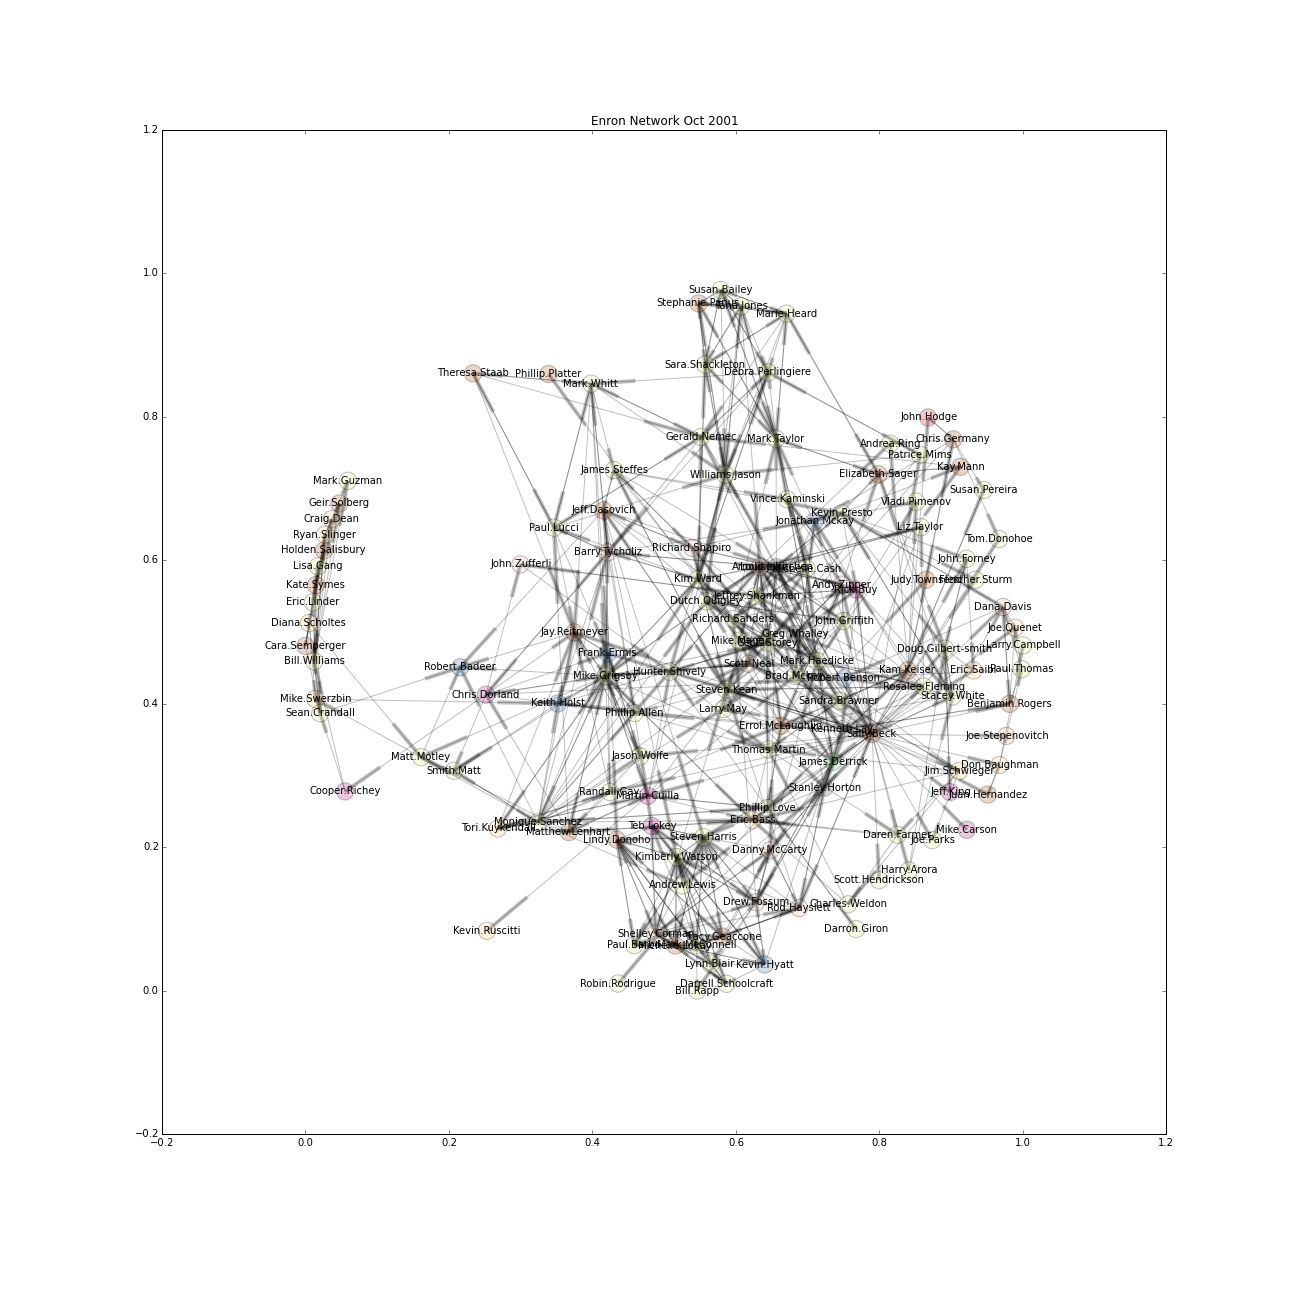
\includegraphics[width=1\textwidth]{figureEnronOct2001}
	\\
	
	\par Terminology used in the rest of the paper
	\beign{enumerate}
	\item $A$ is the adjacency matrix of the network which is $n x n$ for a network with $n$ nodes.
	\item $D$ is the diagonal matrix containing node degrees on it's diagonals
	\item $L$ is the laplacian of the matrix defined as $D - A$
	\item $B$ Is the modularity matrix defined as $B_{ij} = A_{ij} - \frac{k_i k_j}{2m}$ where $k_a$ is degree of node $a$
	
	\end{enumerate}

\section{Centrality Measures} One of the key questions one can ask about an information network such as the Enron email network is: Who are the most important actors in the network? There are various measures of centrality one can use to answer that question.
	\subsection{Eigenvector Centrality} Eigenvector based centrality measures are based on the idea that a node is important if it is connected to other important nodes. Let $A$ be the adjacency matrix of a graph and $x$ the vector of centrality measures. We would like the centrality of each node to be proportional to the centralities of all the nodes connected to it. In matrix form then we would like vector $x$ to satisfy the 
		\begin{equation}
			A x = \kappa x
		\end{equation}
		Thus $x$ is an eigenvector of the matrix $A$. Even though all eigenvectors of $A$ satisfy the above equation, the eigenvector corresponding to the largest eigenvalue is used in practice. \\
		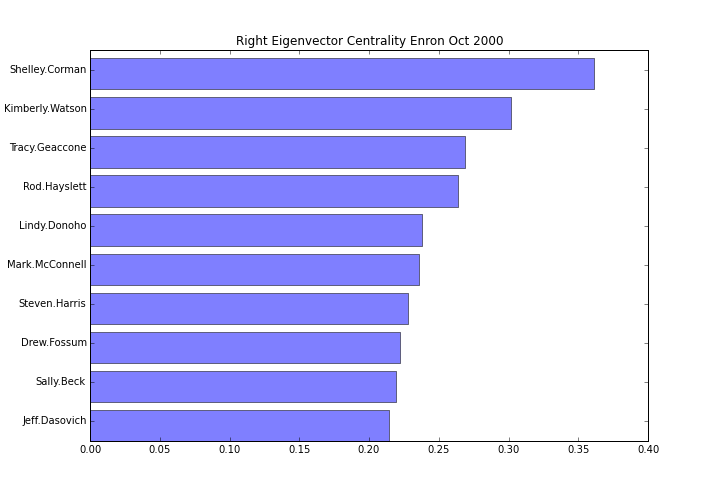
\includegraphics[width=0.7\textwidth]{figureRightEigOct2000} \\
		\\
		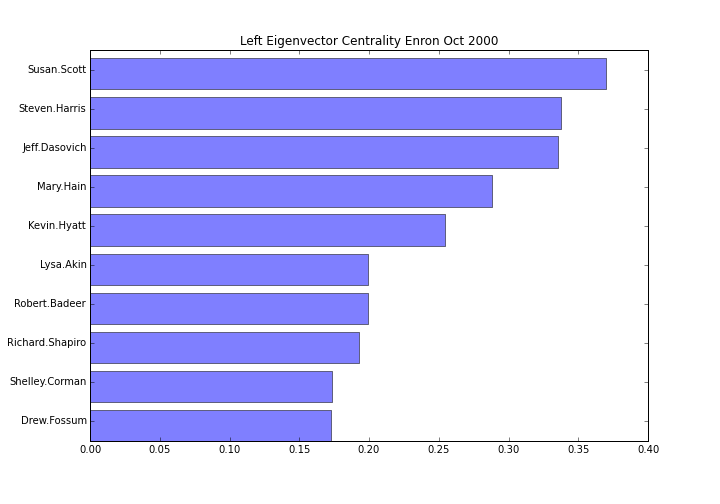
\includegraphics[width=0.7\textwidth]{figureLeftEigOct2000} \\
		
		Two people with very high Eigenvector centrality are Shelley Corman who was Vice President of Regulatory Affairs and Jeff Dasovich who was a Government Relations Executive. It is interesting that two of the most central members of this network are people interfacing between Enron and it's regulators. Susan Scott's (the person with the highest score) role at Enron is not known.\\ \\
		
		Katz Centrality and PageRank are slight modifications of the eigenvector centrality idea.
	
	\subsection{Other measures of Centrality} Why might they be useful
	\begin{enumerate}
	\item In and Out degree
	\item Betweenness centrality
	\end{enumerate}

\section{Communities} Brief background on homophily and measures of it on a graph. \\ \\
	\par Modularity is measure of homophily in the network. The idea is that we find  the fraction of edges that run between vertices of the same type, and then we subtract from that figure the fraction of such edges we would expect to find if edges were positioned at random without regard for vertex type \cite{networkBook}. When the fraction of edges between vertices of the same type is significantly greater than what would be expected at random, we can say that the network exhibits high homophily. The number of edges that run between nodes of the same type is given by
	\begin{equation}
		\sum_{edges (i,j)} \delta (c_i, c_j) = \frac{1}{2} A_{ij} \delta (c_i, c_j)
	\end{equation}
	where $A$ is the adjacency matrix, $c_i$ and $c_j$ are the classes of nodes and $\delta (m,n)$ is the Kronecker delta which is equal to 1 if $m = n$ and 0 otherwise.
	\par The expected number of edges between nodes of the same type is given by
	\begin{equation}
		\frac{1}{2} \sum_{i,j} \frac{k_i k_j}{2m} \delta (c_i,c_j)
	\end{equation}
	where $k_i$ denotes the number of edges of node $i$ (it's degree) and $m$ is the total number of edges in the network. Subtracting (3) from (2) gives us modularity $Q$
	\begin{equation}
		Q = \frac{1}{2m} \sum_{i,j} \left( A_{ij} - \frac{k_i k_j}{2m} \right) \delta (c_i,c_j)
	\end{equation}
	
	Modularity of the Enron graph:
	
	\subsection{Spectral Partitioning} 
		This is is summary of the method described in \cite{networkBook}. 
		Laplacian of the graph. Why is it important.  \\
		How can we use the second lowest eigenvector of the laplacian to split the partition. \\
		Application to the Enron dataset \\
	\subsection{Modularity Maximization Using Spectral Techniques} 	
		Modularity matrix \\
		Maximization Problem and solution using Lagrangian \\
		Communities found in the Enron Dataset 
	\subsection{Singular Value Decomposiiton}
		Low Rank Approximation of Martix \\
		Community Detection using SVD \\

\section{Evolution Across Time} How various  features have evolved over time

\section{Conclusion}

\begin{thebibliography}{9}

\bibitem{shetty}
Shetty, J., Adibi, J. (n.d.). The Enron Dataset
Database Schema and Brief Statistical Report

\bibitem{pfeiffer}
https://www.cs.purdue.edu/homes/jpfeiff/enron.html
data retrieved on Nov 11 2014

\bibitem{nyt}
http://www.nytimes.com/2006/01/18/business/worldbusiness/18iht-web.0117enron.time.html

\bibitem{park}
http://cis.jhu.edu/~parky/Enron/employees

\end{thebibliography}

\end{document}
